
\chapter{Introduction} 

\label{Chapter1} 

\section{Software Transactional Memory}
\label{STMInterface}
Software Transactional Memory (STM in the following) is a programming language independent synchronization concept. Today STM is available 
in all common programming languages\footnote{Even though STM is language independent, I will present the STM library in Haskell since this thesis is
about STM in Haskell}. To understand the benefits of STM, take a look at the following example:
\begin{lstlisting}
type Account = MVar Int

transfer :: Account -> Account -> Int -> IO ()
transfer src dst am = do
  balSrc <- takeMVar src
  balDst <- takeMVar dst
  putMVar src (balSrc - am)
  putMVar dst (balDst + am)
\end{lstlisting}
This is a simple implementation of a bank account and an associated transfer function. This implementation uses an \code{MVar}
for synchronization. An \code{MVar} is a buffer with a capacity of one. This buffer can either be empty or filled. If the MVar is empty,
every \code{takeMVar} operation on this MVar blocks until it is filled. If the MVar is filled, \code{takeMVar} empties the 
\code{MVar} and return the value. \code{putMVar} is the opposite operation. It fills the MVar with a value, if it is empty and 
suspends if the MVar is already filled.

This means \code{transfer} first empties both \code{Accounts}, then modifies the balances and at last writes back the new balances.
At first glance this function seems to work fine, but the following example contains a deadlock:
\par\noindent
\begin{minipage}[t]{.45\textwidth}
Thread 1:
\begin{lstlisting}[frame=lrtb]
main = do
  transfer acc1 acc2 50
\end{lstlisting}
\end{minipage}
\hfill
\begin{minipage}[t]{.45\textwidth}
Thread 2:
\begin{lstlisting}[frame=lrtb]
main = do
  transfer acc2 acc1 50
\end{lstlisting}
\end{minipage}

The problem is the mutual access of the MVars. If both threads take their \code{src} at the same time, they will both wait for \code{dst}
\footnote{In fact is \code{transfer acc1 acc1 50} enough to evoke a deadlock}. To avoid this deadlock we can rewrite the code:
\begin{lstlisting}
transfer src dst am = do
  srcBal <- takeMVar src
  putMVar src (srcBal - am)
  dstBal <- takeMVar dst
  putMVar dst (dstBal + am)
\end{lstlisting}
This indeed solves the problem regarding the deadlock. In return we lose consistency. For a brief moment we see an inconsistent state. Since
the amount is allready subtracted from one account, but not yet added to the other account. This inconsistent state is observable by other 
threads. This is not possible in the first implementation. 

We can use STM to avoid these problems. STM provides a single element buffer named \code{TVar}. A TVar always holds an value and is never 
empty. TVars are read and written with the functions \code{readTVar} and \code{writeTVar}, respectively. 
In contrast to \code{putMVar} and \code{takeMVar}, the TVar operations are not \code{IO} actions but \code{STM} action\footnote{If 
you are wondering when I use \code{SMT} and when STM. I use \code{STM} when I refer to the Haskell type constructor and STM when I refer to STM as library}. 
\code{STM} is an instance of Monad, hence multiple \code{STM} actions can be combined
using the comfortable do-notation. The following code represents the example from above implemented with TVars instead of MVars:
\begin{lstlisting}
type Account = TVar Int

transfer :: Account -> Account -> Int -> STM ()
transfer src dst am = do
  srcBal <- readTVar src
  dstBal <- readTVar dst
  writeTVar src (srcBal - am)
  writeTVar dst (dstBal + am)
\end{lstlisting}
Note the type of transfer is no longer an \code{IO} action, but an \code{STM} action. Apart from this the code looks
similar to the MVar version.

In order to execute a transaction the function \code{atomically :: STM a -> IO a} is used. 
Since \code{readTVar} and \code{writeTVar} do not lock the TVar, the following example contains no deadlock:
\par\noindent
\begin{minipage}[t]{.45\textwidth}
Thread 1:
\begin{lstlisting}[frame=lrtb]
main = do
  atomically $
    transfer acc1 acc2 50
\end{lstlisting}
\end{minipage}
\hfill
\begin{minipage}[t]{.45\textwidth}
Thread 2:
\begin{lstlisting}[frame=lrtb]
main = do 
  atomically $ 
    transfer acc2 acc1 50
\end{lstlisting}
\end{minipage}

This is because STM ensures the \keyword{ACID} properties. The ACID properties were Introduced in \parencite{DBTrans} for
database transactions. These properties were adapted for software transactions later on.
In the case of software transactions the ACID properties mean the following:
\begin{itemize}
 \item \keyword{Atomicity}: the transaction executes all operations or none.
 \item \keyword{Consistency}: all modifications of a transaction are committed at the same time. No transition state is observable.
 \item \keyword{Isolation}: no concurrency is observable by a transaction. Each transaction can work as if it is the only transaction.
 \item \keyword{Durability}: ensures the perseverance of the changes. In the case of software transactions this is not necessary.
\end{itemize}
These properties explain the name \code{atomically}, because the enclosed code appears to be executed instantaneously without any 
interactions with other threads.
Before we turn over to the implementation of STM, we take a deeper look at the interface of the STM.

\code{newTVar :: a -> STM (TVar a)} creates a newTVar. Since a TVar always holds a value, an initial value has to be
passed to create a TVar. There is no function like \code{newEmptyTVar}. 

Besides functions to create and access TVars, there are functions to alter the control flow.
\code{retry :: STM a} is a generic STM action that indicates a failure, thus whenever a transaction engages a \code{retry} it restarts. The transaction
is \textbf{not} restarted immediately. The transaction restarts, if at least one of the TVars it has read is modified. If the transaction would
restart immediately (and no TVar has changed), the transaction would run into the same \code{retry} again. 

With \code{orElse :: STM a $\rightarrow$ STM a $\rightarrow$ STM a} you are able to express alternatives. \code{orElse} executes the first transaction
and ignores the second transaction, if the first transaction is successful. If the first transaction fails (retries), the second transaction is 
executed instead.

Note that it is not possible to execute \code{IO} action within a transaction, which means that not side effects can occur. Furthermore this means
restarting a transaction will never lead to the re-execution of irreversible operations. The reason is that the computations of transactions
are done within the \code{STM} Monad. In other words the type system of Haskell forces us to write correct transactions. 

For single threaded programming, abstraction and composability are key features. These features allow us to combine smaller pieces
of code into more complex pieces of code. These feature are not available for lock based concurrent programming. Compose correct lock based
concurrent functions most likely lead to deadlocks or inconsistencies. Consider the following example:
\begin{lstlisting}
withdraw :: Account -> Int -> IO()
withdraw acc am = do 
  bal <- takeMVar acc 
  putMVar acc (bal - am)
 
deposit :: Account -> Int -> IO()
deposit acc am = withdraw acc (-am)
\end{lstlisting}
These are functions to withdraw and deposit money from and on an account. The natural way to implement \code{transfer} is:
\begin{lstlisting}
transfer :: Account -> Account -> Int -> IO()
transfer src dst am = do
  withdraw src am
  deposit dst am
\end{lstlisting}
We reuse the functions that are already defined instead of coding everything from the scratch. In our example this is equivalent 
to the solution suggested above to eliminate the deadlock. This implementation is free of deadlocks, but it lacks consistency.
Thus building complex concurrent operations can not take advantage of abstraction and composability. We always need to code
everything from the scratch. This is error prone in compared to the step wise combination of smaller operations into 
bigger operations.

STM allows us to use this important programming paradigm for concurrent programming. Thus the following example provides
deadlock freedom as well as consistency.
\begin{lstlisting}
withdraw :: Account -> Int -> STM()
withdraw acc am = do 
  bal <- readTVar acc 
  writeTVar acc (bal - am)
 
deposit :: Account -> Int -> STM()
deposit acc am = withdraw acc (-am)

transfer :: Account -> Account -> Int -> STM()
transfer src dst am = do
  withdraw src am
  deposit dst am
\end{lstlisting}
We can combine arbitrary transactions to more complex transactions while preserving the ACI properties. This greatly benefits the 
readability of the code. In addition it increases the efficiency of the development process, because we are able to reuse code
that we already found to be correct. This was also one of the main motivations of paper \parencite{STMBase} which forms the foundation
of STM in Haskell.

  
\section{Implementation}
In this we explore the current implementation of STM in Haskell, more specific in GHC. For a detailed description of the implementation 
refer to \url{https://ghc.haskell.org/trac/ghc/wiki/Commentary/Rts/STM}. 

Even though the current implementation uses a low level C-library, we retain an abstract view on the implementation, since the technical 
details are not important for the course of this thesis. An abstract view on the implementation is presented to understand how the ACI 
properties are ensured.

The execution of a transaction (a call of \code{atomically}) is split in two phases. First the computation phase and second the commit phase. 
 
\subsection{Computation Phase}
Each transaction holds a log for the TVars it has accessed. The log contains four elements per entry. These are: 
\begin{itemize}
 \item tvar
 \item expectedValue
 \item newValue
 \item versionNumber
\end{itemize}
The \code{versionNumber} is only used to prevent a very subtle bug and thus not considered in this thesis. 
The log is extenden and modified by the transactional operations \code{writeTVar} and \code{readTVar}. \code{newTVar} on 
the other hand creates the new TVar directly. Whenever \code{readTVar} is called the associated TVar is lookep up in the log.
If it is present, the \code{newValue} is returned. If it is not present, a new entry for the log is created. While \code{tvar}
is the passed TVar, \code{newValue} and \code{expectedValue} are the actual value of the TVar and \code{versionNumber} is 
the actual verison number.
This is the one of the two times in the computation phase when the transaction accesses the actual mutable data structures.  
After the entry is created and added to the log, the actual value is returned. 

A call of \code{writeTVar} also looks up the associated TVar in the log. If it is present, the field \code{newValue} is 
set to the value passed to writeTVar. If it is not present, a new entry is created. The \code{tvar} is the passed TVar and
the \code{newValue} is the passed value and \code{expectedValue} is the actual value of that TVar. This is the other time 
the actual mutable data structures are accessed in the computation phase. 

This log fulfills two purposes. One purpose of the log is the use in the commit phase which is described in \ref{Sec:STMImpl}.
The other is the interaction between \code{readTVar} and \code{writeTVar}. The \code{readTVar} operations are able to see the results 
of preceding \code{writeTVar} operations in the log. Without the log \code{writeTVar} would need to access the actual TVar. This on the 
other hand would imply that other transactions would be able to see inconsistent intermediate states of the system;
a violation of the ACI properties. It may seem unnecessary to read a TVar that the transaction itself wrote before.
The transaction should know what it writes and thus does not need to access such TVars. Nevertheless there are two reasons 
to allow it. The current implementation allow the user to combine all transactional actions in an arbitrary manner and 
the library ensures (at compile time) that it works correctly. To restrict the user to only read TVars he has
not yet written, no longer allows the library to give this kind of guarantee at compile time; this contradicts
the design concept of Haskell. The second reason is one of the core motivations of STM in Haskell: composability.
With the restriction it is not possible to combine arbitrary correct STM functions to new more complex STM
functions. 

Take a look at the following example:
\begin{lstlisting}
transaction = do
  a <- readTVar t1
  b <- readTVar t2
  writeTVar t1 b
  writeTVar t2 a
\end{lstlisting}
This code would lead to the following log:
\begin{lstlisting}
 log  = {(t1,a,b),(t2,b,a)}
\end{lstlisting}
The log contains two entries, because the transaction accessed two TVars. The first entry contains the information that \code{t1}
hold the value \code{a} when it was first read and the value \code{b} is the new value of it. \code{t2} hold the value \code{b} 
and the new value is \code{a}. Before we will examine the commit phase, we will look at the other operations of the STM interface.

\code{newTVar} creates a new TVar and initializes this TVar. Afterwards this TVar can be used like already existing TVars.
Even if the transaction is rolled back, the new created TVars are not deleted explicitly. This work is done by the garbage
collector, since the TVars are not further referenced, if the transaction that created them is rolled back. 

\code{retry} aborts the computation and returns a results that indicates a failure. This result may be intercepted by 
\code{orElse} or is passed to \code{atomically} directly. 

If \code{atomically} receives an result that indicates an failure, it aborts the transactions. 
Aborting a transaction means to discard the log. Since no observable operations are performed in the computation phase, nothing has to be undone. 
As soon as at least one of the TVars in the log has changed, the transaction is restarted. If the transaction is restarted immediately and no 
TVar has changed the transaction would reach the same \code{retry} again. These changes can be checked by comparing the \code{expectedValue} in
the log with the actual value in the TVar. To avoid busy waiting the thread do not repeatedly check if the value has changed. The TVar has a 
queue for wait waiting threads. Each time a transaction successfully commits and writes a TVar it also checks if there is someone waiting in 
this queue. The committing thread then notifies all waiting threads.

\code{orElse} on the other hand reacts differently on the the result that indicates a failure. The implementation works with nested transactions, 
but to explain this in detail would go beyond the scope of this thesis. Nested transactions are not able to publish their writes on their own.
When a nested transaction successfully commits(we see in the next section what this means), its log is integrated in the log of the surrounding transaction. 
Integrated means the logs are merged and in the case one entry is in both log the entry of the outer transaction is discarded.
If the nested transaction fails, because \code{retry} occurred and it is the first transaction of \code{orElse}, the log of the inner transaction
is integrated in the log of the surrounding transaction, but the \code{newValue} fields of the inner log are ignored. If the nested transaction
fails to validate the outermost transaction is rolled back.

In conclusion the interface functions of STM are processed in the computation phase as follows:
\begin{itemize}
 \item \code{writeTVar}: Look up TVar in log. If present update \code{newValue}. If not present read actual TVar and create new entry.
 \item \code{readTVar}: Look up TVar in log. If present return \code{newValue}. If not present read actual TVar and create new entry.
 \item \code{newTVar}: Create and initialize a new TVar. 
 \item \code{retry}: Return a result that indicates a failure.
 \item \code{orElse}: Create a nested Transaction and reacts on the return value of that transaction.
\end{itemize}

\subsection{Commit Phase}
\label{Sec:STMImpl}
After the log is calculated and no further STM actions need to be processed, the commit phase starts.
At first the transaction validates if the values in its log are still correct by \keyword{validating} its log.
Validation denotes the process to check if the expectedValues are equal to the actual values in the TVars.
In other words for each entry in the log the transaction reads the actual TVar and compares the value with 
the \code{expectedValue} in the log. If at least one of these values does not match, the transaction is considered
\keyword{invalid}. If the validation returns the transaction is instantaneously rolled back, by discarding the log 
and restart it computation. If all values match the the transaction is considered \keyword{valid}. If the validation
returns valid, each entry in the log is processed. 

If \code{expectedValue} differs from \code{newValue} the associated TVar is locked. The transaction has acquired all 
locks it needs, it validates again. This seems a bit wasteful in terms of resources, but locking the TVars is considered
an expensive operation and thus the implementation tries to avoid this when ever possible. This process reduces the chance
that the transaction acquires all locks and then finds out it is invalid and consequently a unnecessary locking of TVars.
If the validation fails at this point, the transaction is rolled back after the locks has been released.
If the transaction has acquired all locks and is valid the transaction is is ready to publish its changes.
This means iterating on the log and update the actual TVars where \code{expectedValue} and \code{newValue} differ and
simultaneously releasing the locks. 

If the validation returns invalid it means at least one \code{expectedValue} is no longer correct. To roll back is essential 
to retain the ACI properties. The failed validation indicates that transaction has read an outdated value and possibly worked 
with this value. Take a look at the following example:
\begin{lstlisting}
transaction = do 
  a <- readTVar t1
  writeTVar t1 (a+1)
\end{lstlisting}
If this transaction is processed by two transactions in parallel. Both would read the initial value of \code{t1}, say \code{1}.
So both would note in their log \code{(t1,1,1)}. After the \code{writeTVar} the log of both transactions would look contain 
\code{(t1,1,2)}. After that both transactions try to commit. Assume one transaction commits before the other transaction tries.
\footnote{For simplicity we assume that no other transaction is running besides the two we are looking at.}
Then the transaction would find its log to be valid and lock \code{t1}. After that its log is still valid and so it modifies 
\code{t1} and releases the log. 
Then the second transaction tries to commit. Since the actual value hast changed to \code{2} it does no longer match 
the \code{expectedValue} and the transaction is rolled back. If the transaction would not be rolled back at this point
and commit instead. The transaction would write \code{2} to the TVar (that already contains \code{2}). In the end 
this would means the value of \code{t1} is \code{2} after both transactions have finished. This is certainly not the 
intended behaviour after incrementing the TVar that holds \code{1} twice. This is the well known \keyword{lost update}
problem. 

By rolling back the second transaction it reads \code{t1} once more. The log contains \code{(t1,2,2)} after the \code{readTVar}
operation and \code{(t1,2,3)} after the \code{writeTVar} operation. Then the transaction validates, locks, validates and 
finally publishes it modifications. In the end the value of \code{t1} is \code{3}; just as intended.

\subsection{Notes on the Implementation}
Larus and Rajwar describe in their book\parencite[Chapter 2]{transBook} different design options to be done when implementing a 
(Software) Transactional Memory. While most of these options effect only the performance of a system, some also effect the 
semantics of the system. We will discuss in this section the design options that are important for this thesis \footnote{The names used in the 
following part are taken from \parencite[Chapter 2]{transBook}}.

\subsubsection{Deferred and Direct Updates} The way a STM system modifies the underlying data structures can either be \keyword{deferred}
or \keyword{direct}. Direct updating systems are writing the actual objects when a write operation is called. In the case of Haskell 
this would mean, every time \code{writeTVar} is called. Deferred updating systems on the other hand buffer the write operations to
commit them later on. Haskell STM is a deferred updating system, since the values are buffered in the writeSet before they are
committed. This design options does not effect the semantics of the system. While a direct system loses performance, when a transaction
is rolled back, because the initial values need to be restored, a deferred systems contains an overhead due to the need to log values
and looking them up. Neither mechanism is better than the other in general; it depends on the application that STM is used in. 
\parencite{pessimisticSTM} compares a deferred and a direct system. They show that the performance of a direct update 
system is significantly higher than that of a deferred system, when reads outnumber writes by far.

\subsubsection{Early and Late Conflict Detection} A STM system needs to detect conflicts in order to ensure the ACI properties. This can 
be done as soon as the conflict occurs or later before the transaction commits. If the system uses a late conflict 
detection, transactions may work on an inconsistent state. This may lead to loops or exceptions. So this design decision is 
relevant for the semantics. Haskell STM uses a late conflict detection. By validating the log before comitting the transaction a possible conflict
is detected. This implies the transaction may work on an inconsistent state until it attempts to commit. This means the transaction 
may run into an infinite loop, because it saw an inconsistent state. To avoid this problem, additional validations are performed
each time the executing thread yields. Exceptions raised by the transaction are handled like a \code{retry}. If the log is valid,
the transcation waits until at least one TVar changed. If it is invalid the transaction is restarted immediately.
In conclusion, the user of STM can not observe that the transaction worked on an inconsistent state.

\subsubsection{Synchronization} The last important property of a STM system is the way it synchronizes transactions. In order to validate
correctly the systems needs to make sure the validation result does not depend on race conditions and is correct until the commit 
is completed. This means either concurrent transactions are delayed or their commit does not change the each others validity. In Haskell the first
approach is taken. When a transaction commits, the TVars in the log that are updated are locked, thus other transactions that may conflict are not 
able to commit at the same time. In order to avoid a deadlock, all locks are released and the transaction
is rolled back when it tries to aquire the lock for a locked TVar. In the worst case this leads to the roll back of both transactions, 
however the chances are narrow. Rolling back the transaction seems to be harsh instead of waiting until the other transaction finishes 
and then trying to commit, but if two transactions try to lock the same TVar, both transactions try to write this TVar. 
This means at least one of the transactions is rolled back, since the TVar is logged with the old value. 
Thus the first transaction to commit would modify a value in the log of the other transcation.

\section{Problems}
In this section we turn over to the problems in the current implementation. These problems can be examined independently. The first problem is about
\textit{when} a transaction is rolled back and the second problem is about \textit{how} a transaction is rolled back.

\subsection{Unnecessary Rollback}
\label{Prob:UnRo}
Remember the STM implementation of \code{transfer} and its example use given in \ref{STMInterface}: 
\par\noindent
\begin{minipage}[t]{.45\textwidth}
\begin{lstlisting}[frame=lrtb]
transaction1 = do
  atomically $
    transfer acc1 acc2 50
\end{lstlisting}
\end{minipage}
\hfill
\begin{minipage}[t]{.45\textwidth}
\begin{lstlisting}[frame=lrtb]
transcation2 = do 
  atomically $ 
    transfer acc2 acc1 50
\end{lstlisting}
\end{minipage}
The implmentation is correct, but not verry efficient in this case. Take a look at the inlined functions to understand the 
problem:
\par\noindent
\begin{minipage}[t]{.45\textwidth}
\begin{lstlisting}[frame=lrtb]
transaction1 = do
  a1 <- readTVar acc1
  a2 <- readTVar acc2
  writeTVar acc1 (a1 - 50)
  writeTVar acc2 (a2 + 50)
\end{lstlisting}
\end{minipage}
\hfill
\begin{minipage}[t]{.45\textwidth}
\begin{lstlisting}[frame=lrtb]
transaction2 = do 
  a1 <- readTVar acc2
  a2 <- readTVar acc1
  writeTVar acc2 (a1 - 50)
  writeTVar acc1 (a2 + 50)
\end{lstlisting}
\end{minipage}

Due to the scheduler the threads can run in a sequential order. This case may occur, but is not desirable. It means 
there is no performce improvement by executing this on multiple cores/processors. Thus the efforts to use multiple
threads are futile in the first place. This is not a problem specific to STM, but to all synchronization mechanisms. 
If the resulting multi threaded program is not scheduled in a way that it is executed parallel, these mechanisms are a
performance deterioration rather than a performance improvement. Since we cannot access the scheduler, we ignore 
this case. 

The second case is that these transactions are run in parallel. This should be the better case, because the implementation
has a chance to improve the performance. Sadly this is not the case. To understand why, we need to take a close look at 
the execution. Let us assume both threads execute their computation phase at the same time. This means both read the initial 
values of \code{acc1} and \code{acc2} and add these information to their log. Furthermore add both transactions 
entries for \code{writeTVar acc1} and \code{writeTVar acc2} to their log. Then both transactions try to commit, thus try to lock 
the TVars. It is possible both transactions are rolled back at this point. Lets assume \code{transaction1} acquires the locks 
for \code{acc1} and \code{acc2}. Since no TVars were modified after \code{transaction1} read them, it validates and commits.
If \code{transaction2} tries to access the TVars before \code{transaction1} has finished committing, it is rolled back. 
Thus it is possible for \code{transaction2} to read the old value once again. If \code{transaction2} is descheduled for the time
\code{transaction1} commits, it is rolled back afterwards, because the values of \code{acc1} and \code{acc2} have were changed 
by \code{transaction1}. In conclusion no performance improvement was achieved. The most efficient execution is if both transactions
are executed in a sequential order. As mentioned before, this not desirable for multithreaded programs.

\begin{figure}
\centering
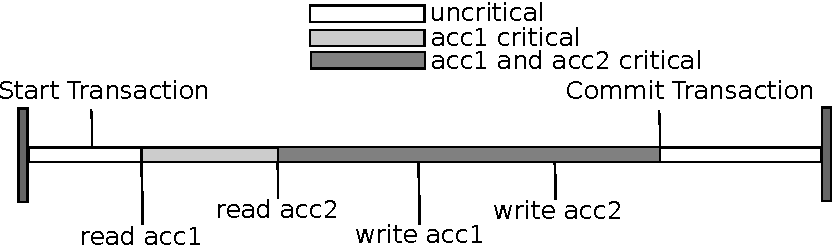
\includegraphics{Figures/CriticalValue}
\decoRule
\caption[CriticalValue]{Time when the update of \code{acc1} or \code{acc2} causes a rollback.}
\label{fig:criticalValue}
\end{figure}

This leads to two questions:
\begin{itemize}
 \item When is it needed to roll back a transaction?
 \item How can we avoid or at least decrease rollbacks?
\end{itemize}
A transaction needs to be rolled back if it is operating on data that is not a snapshot of the current memory. In other words 
if a value has changed after the transaction read this value. When a transaction reads a TVar, this TVar becomes 
\keyword{critical} for the transaction. Critical means a modifications of that TVar causes the transaction to roll back.
Figure \ref{fig:criticalValue} visualizes when the TVars \code{acc1} and \code{acc2} are critical for \code{transaction1}.
When \code{readTVar acc1} is executed the values becomes critical and stays critical until the transaction commits.
If any other transaction commits a modification to \code{acc1} or \code{acc2}, while \code{acc1} and \code{acc2} are
critical for \code{transaction1}, \code{transaction1} is rolled back to preserve the ACI properties. A solution other
than the roll back is presented in \ref{Prob:UnRe}. 

This insight brings an intuitive way to deal with this problem. If we minimize the time the TVars are critical for
a transaction we reduce the chance that this transaction is rolled back. 
If we rearrange the operations of \code{transfer}, we are able reduce the time \code{dst} is critical. Note that we 
can rearrange the operations to a certain degree without changing the semantics of the resulting code due to the ACI 
properties. 
\begin{lstlisting}
transfer src dst am = do 
  srcBal <- readTVar src
  writeTVar src (srcBal - am)
  dstBal <- readTVar dst
  writeTVar dst (dstBal - am)
\end{lstlisting}
With this implementation of transfer the time in that both TVars are critical is reduced. Figure \ref{fig:criticalValue2}
shows the effects of this for \code{transaction1}. The second TVar, namely \code{acc2}, is shorter critical than in the 
initial implementation. The time \code{acc1} is critical has not changed at all. Nevertheless it shows that delaying the
execution of \code{readTVar} can reduce the time values are critical and by this the chance the transaction is rolled back.
\begin{figure}
\centering
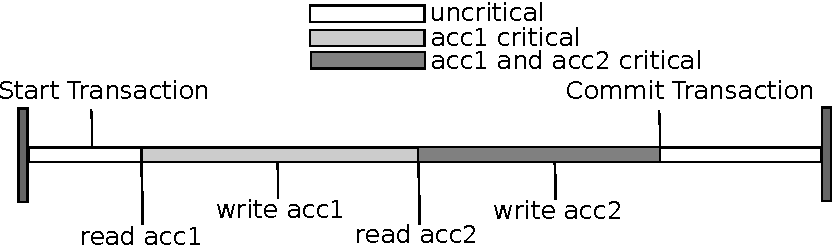
\includegraphics{Figures/CriticalValue2}
\decoRule
\caption[CriticalValue2]{Effect of rearranging code with regards to the time \code{acc1} and \code{acc2} are critical for \code{transaction1}.}
\label{fig:criticalValue2}
\end{figure}
Our aim is to delay the execution of \code{readTVar} as far as possible to reduce to time that
a TVar is critical for the transaction. We have already seen one option to achieve this; rearrange the 
operations of a transaction. This would require a kind of preprocessing in the compiling process, for 
example a source to source code transformation. The aim of this thesis is to provide an pure Haskell
library. I do not intend to implement an extension to the compiler nor do I 
want to provide a source to source code transformer. The only other option is to alter implementation
of \code{readTVar} and \code{writeTVar} without changing the \keyword{external} semantics of STM. 
External semantics are the semantics the user can observe and which effect the user written code.

The critical time would be minimal if the TVars were read directly before or at the start of the commit phase.
This would mean the chances that another transaction commits a change to a TVar that is critical are low or non
existing. So the idea is to let the user define transactions like before, but changing the semantics of 
\code{readTVar} that it is evaluated in the commit phase. The user is able to define transactions like with 
the original implementation, but the delay of the evaluation shortens the time TVar are critical and thus
the chance a transaction is rolled back. 

If we refer to our example: 
\par\noindent
\begin{minipage}[t]{.45\textwidth}
Thread 1:
\begin{lstlisting}[frame=lrtb]
transaction1 = do
  a1 <- readTVar acc1
  a2 <- readTVar acc2
  writeTVar acc1 (a1 - 50)
  writeTVar acc2 (a2 + 50)
\end{lstlisting}
\end{minipage}
\hfill
\begin{minipage}[t]{.45\textwidth}
Thread 2:
\begin{lstlisting}[frame=lrtb]
transaction2 = do 
  a1 <- readTVar acc2
  a2 <- readTVar acc1
  writeTVar acc2 (a1 - 50)
  writeTVar acc1 (a2 + 50)
\end{lstlisting}
\end{minipage}

If we change the semantics of \code{readTVar} by delaying the evaluation, the following happens.
Both transactions will execute the computation phase simultaneously. This means \code{transaction1} adds
\code{(acc1,a1,(a1 - 50))} and \code{(acc2,a2,(a2 + 50))} to its log (this is analog for \code{transaction2}).
At the first glance this seems to be incorrect since the values of \code{a1} and \code{a2} are not yet present.
For Haskell this is quite common. Haskells is a non-strict language, which means passing unevaluated expressions
is normal. 

After the computation phase the commit phase follows. The first step is to lock the read TVars in order to 
perform the validation. Since both transactions used the same TVars, they will commit successively instead of
parallel. 

Assume \code{transaction1} gets the locks first and tries to validate\footnote{You could argue that 
evaluating \code{readTVar} operation is necessary before validating, but this would not change the validity of the 
transaction, since the TVars are locked and can not be modified by other transactions at that point.}. 
Since the readSet contains an action whose result is the current value, the validation is unnecessary; it is always valid.
To validate the log, \code{a} and \code{b} are evaluated. At last the new values are written to the TVars.

After \code{transaction1} finished and released the locks, \code{transaction2} aquires these locks
and validates. The log of \code{transaction2} is also valid and also commits its changes.

Both transactions run parallel as far as possible and did not roll back. Chapter \ref{Chapter2}
presents the limitations of this idea and the challenges that arise when implementing it.

\subsection{Unnecessary Recomputations}
\label{Prob:UnRe} 	
While the first problem dealed with then question \textit{when} transactions need to be rolled back,
the second problem investigates the question \textit{how} transactions are rolled back. Lets take a 
look at our well known example:
\begin{lstlisting}
transfer src dst am = do 
  srcBal <- readTVar src	
  writeTVar src (srcBal - am)	
  dstBal <- readTVar dst	
  writeTVar dst (dstBal + am)	
\end{lstlisting}
This transaction contains two independent statements. The first two lines of the transacton form the first 
statement. This is independent of the last two lines. Independent means their side effects or results do not 
influence each other. While the first line influces the second line, it does not influence the last two lines
and vice versa. 

If the transaction is executed, it computes its log first. Then it locks the TVars and 
validates\footnote{We want study the two problems independently and thus assume the original implementation here.}. 
The validation fails if either of the TVar has changed after it was read by the transaction.
If the validation fails the transcation is rolled back. Which means the log is discarded,
regardless which TVar was the reason for the failed validation. 

Suppose a \code{transaction1} executes \code{transfer acc1 acc2 5} and is deschedules before committing.
Then \code{transaction2} modifies \code{acc1} (and nothing else) and commits. This would cause \code{transaction1}
to roll back and execute both parts of \code{transfer} again. This includes the read and write of \code{t2}, although 
the \code{t2} was not modified. Hence the exact same code with same inputs and the same (relevant) environment 
is executed twice. If we just execute the parts of a transaction that are invalid instead of all, we can save a 
considerable amount of time when a transaction is rolled back. This means for the exmple, it is enough to remove 
the entry for \code{acc1} from the log an execute the first two actions of transfer instead of all actions.

This concludes the overview on the problems of the current STM implementation. We will now turn over to the 
solution for this problems.







% This is the frist phase of a transaction execution. In this phase the reads and all pure calculations are performed. 
% Aforementioned IO action cannot be executed within a transaction, but pure computation may be executed like the following
% example demonstrates:
% \begin{lstlisting}
% transaction = do 
%   val <- readTVar t
%   if f val 
%     then writeTVar t (g val)
%     else retry
% 
% f v = some calculations...    
% g v = some other calculations...
% \end{lstlisting}
% Thus even if the calculation of \code{g} can be delayed thanks to laziness, the calculation of f has to be performed within that transaction.
% The results of \code{f} effects the control flow and thus needs to be evaluated to determine the result of the branch statement. 
% 
% Since 

